\question{Задача о перпендикуляре.}

\begin{figure}[H]
    \begin{center}
      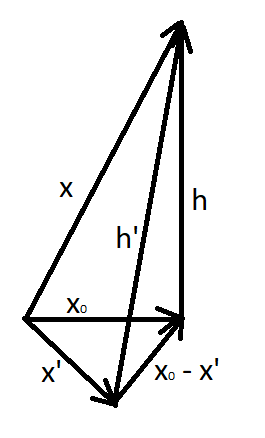
\includegraphics[width=100pt]{LA/Pifagor.png}
    \end{center}
\end{figure}

\textit{Задача.  } Требуется найти перпендикуляр $h: x_0 + h = x$ ($h = x - x_0$), то есть нужно найти точку $M_0$ - 
проекцию $M$ или вектор $x_0$ - ортогональная проекция $X$ на $G$.

\begin{remark}
    $h$ задаёт кратчайшее расстояние $MM_0$ (доказательство ниже)
\end{remark}

\begin{theorem}
    $x_0$ - ортогональная проекция $x$ на $G$, $h=x-x_0$, $h \perp G$, $x_0 \in G$, $x \in E^n$
    
    Тогда $h$ задаёт кратчайшее расстояние от $x$ до $G$, то есть $\forall x' \in G \neq x_0 \,\,\, ||x-x'|| > ||x-x_0||$ 
\end{theorem}
\begin{proof}
    Так как $x', \, x_0 \in G$, то $-x'+x_0 \in G$. Так как $h = x - x_0 \perp G$, то $h \perp (-x' + x_0)$
    \begin{lequation}
        |||x-x'||^2 = ||\underbrace{x - x_0}_{n} + x_0 - x'||^2 = \, \text{(Пифагор)} \, ||x-x_0||^2 + ||x_0-x'||^2 > ||x-x_0||^2 \, (\neq, \text{т.к. } x' \neq x_0) \\
        ||h'|| > ||h|| \, \text{(длина наклонной больше длины перпендикуляра)}
    \end{lequation}
    \begin{remark}
        Это проекция $x$ на $G$, отстоящая от $x$ на наименьшее расстояние
    \end{remark}
\end{proof}

\textit{Вычисление. } Ортогональная проекция $x_0$

$x \in E^n$, $G \subset E^n$, $x_0$ - ортогональная проекция $x$ на $G$

Найти $x_0$ значит найти $x_0=\lambda_{1}e_{1} + \dots + \lambda_{k}e_{k}$, 
где $\{e_1, \dots, e_k\}$ - базис $G$ (не обязательно ортонормированный). 

Перпендикуляр $h = x-x_0 \perp G \implies (h, e_i) = 0$, то есть $(x-x_0, e_i) = (x, e_i) - (x_0, e_i) = 0$

Таким образом, $(x_0, e_i) = \lambda_1(e_1, e_i) + dots + \lambda_k(e_k, e_i) = (x, e_i)$

$i = 1 \dots k \implies$ получаем СЛАУ k-ого порядка, где неизвестны $\lambda_1 \dots \lambda_k$ - 
коэффициенты $a_{ji} = (e_j, e_i)$

В матричной форме:
\begin{lequation}
    .\text{Матрица Грама } g = \begin{pmatrix}
        (e_1, e_1) & \dots & (e_k, e_1) \\
        & \dots & \\
        (e_1, e_k) & \dots & (e_k, e_k)
    \end{pmatrix} 
    \begin{pmatrix}
        \lambda_1 \\ 
        \dots \\
        \lambda_k
    \end{pmatrix} =
    \begin{pmatrix}
        (x, e_1) \\
        \dots \\
        (x, e_k)
    \end{pmatrix}
\end{lequation}

По теореме Крамера существует единственное решение (определитель $ g \neq 0$)